\chapter{系统设置}%
\label{cha:settings-system-appendix}

\section{VirtualBox 虚拟机}%
\label{sec:vbox-appendix}

\subsection{故障排除}%
\label{sub:vim-troubleshooting}

\subsubsection{gVim 打开文件后不见光标}%
\label{ssub:vim-ts-cursor}

\begin{enumerate}
    \item 最大化虚拟机窗口(参见
        \S\ref{ssub:vbox-set-window-size})后打开文件,
        若能见光标就停止,否则进入下一步。
    \item 打开 \lstinline{~/.gvimrc_customized}, 修改
        \lstinline{linespace} 的设置。比如,可以尝试  \lstinline{0 - 4}
        之间的一个值。
\end{enumerate}

\subsection{图解操作}%
\label{sub:vbox-graphic-illustration}

\subsubsection{设定共享目录的图示}%
\label{ssub:vbox-set-share-folder-a}

\begin{figure}[!htbp]
  \centering
  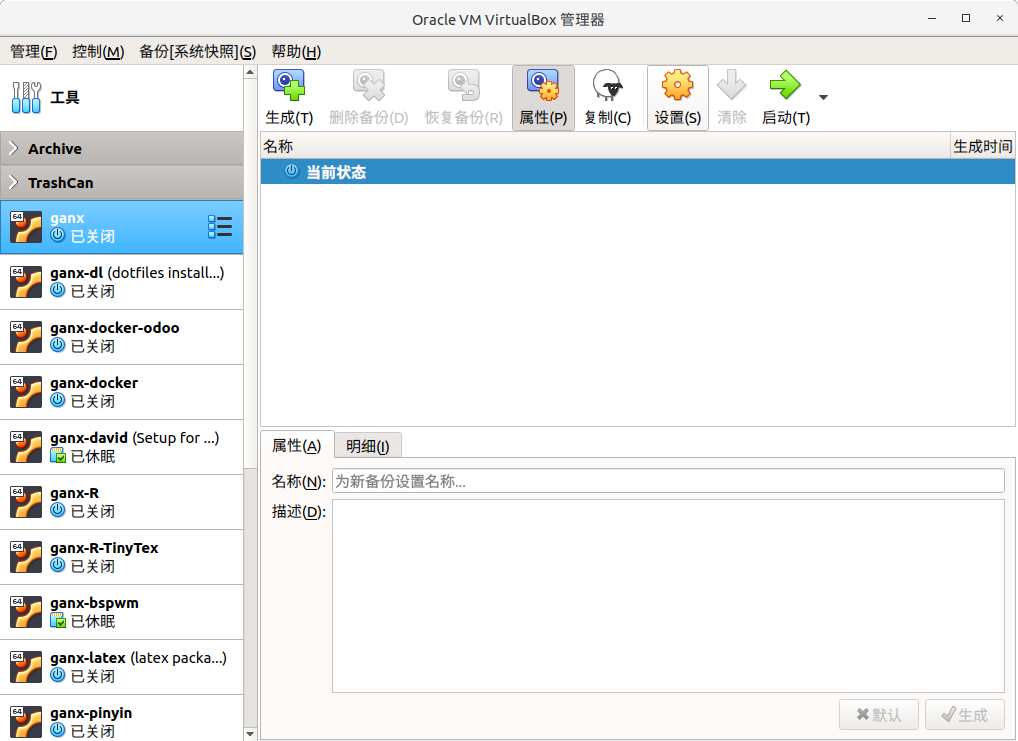
\includegraphics[width=0.9\textwidth]{media/shots/vm/Screenshot from 2019-11-29 17-52-45.png}
  \caption{设定共享目录 --- 示意图 1}
\end{figure}
\begin{figure}[!htbp]
  \centering
  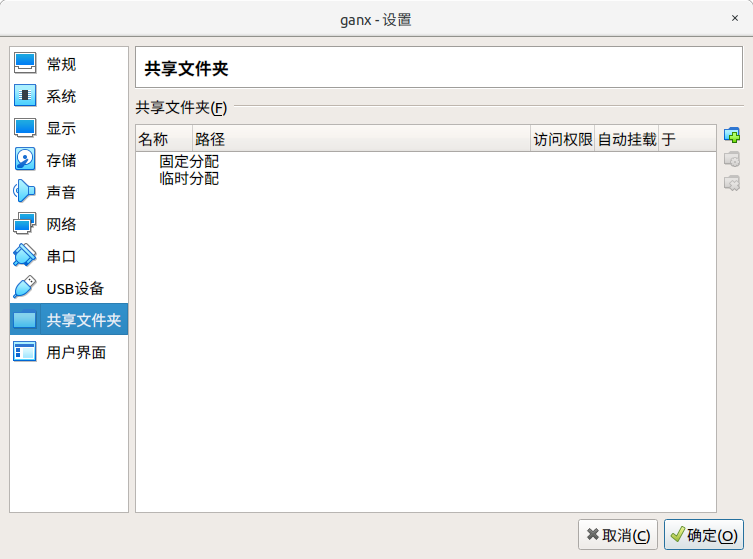
\includegraphics[width=0.9\textwidth]{media/shots/vm/Screenshot from 2019-11-29 17-53-28.png}
  \caption{设定共享目录 --- 示意图 2}
\end{figure}
\begin{figure}[!htbp]
  \centering
  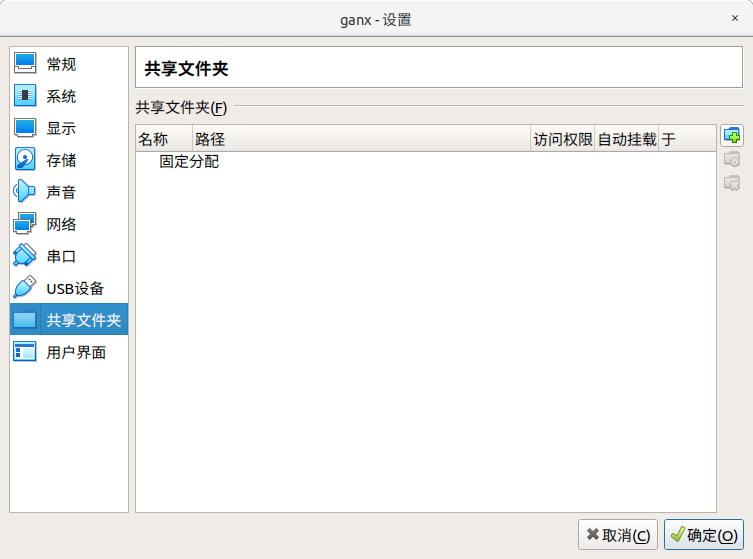
\includegraphics[width=0.9\textwidth]{media/shots/vm/Screenshot from 2019-11-29 17-54-41.png}
  \caption{设定共享目录 --- 示意图 3}
\end{figure}
\begin{figure}[!htbp]
  \centering
  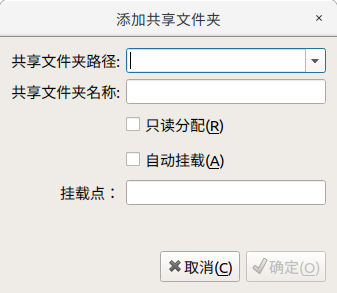
\includegraphics[width=0.9\textwidth]{media/shots/vm/Screenshot from 2019-11-29 17-55-59.png}
  \caption{设定共享目录 --- 示意图 4}
\end{figure}
\begin{figure}[!htbp]
  \centering
  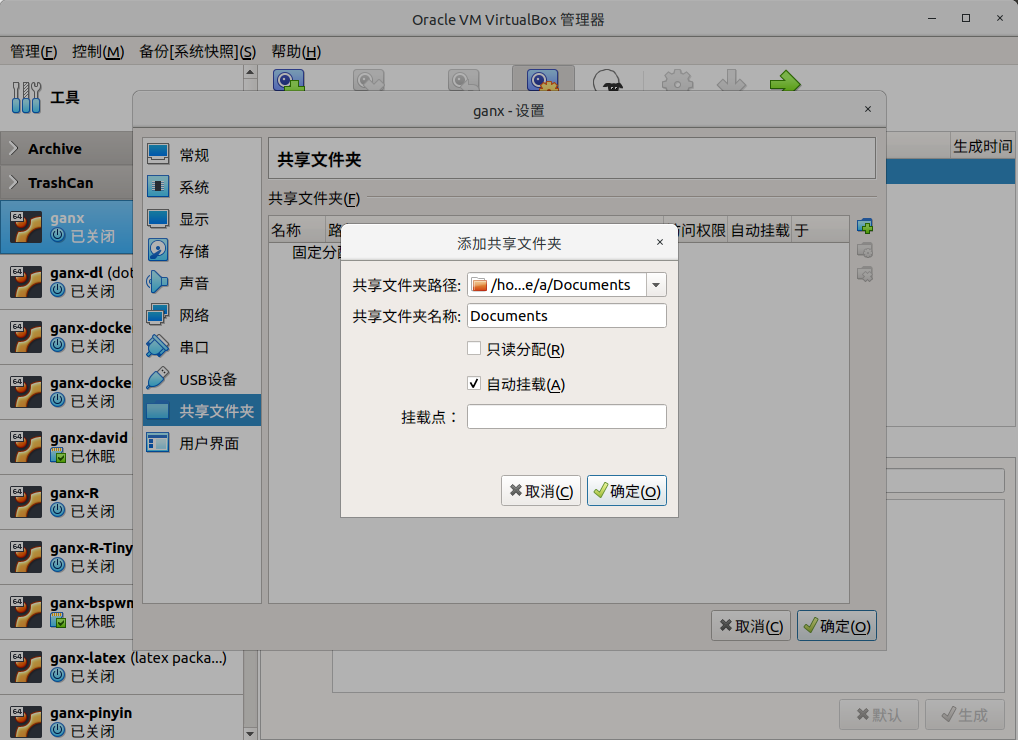
\includegraphics[width=0.9\textwidth]{media/shots/vm/Screenshot from 2019-11-29 17-59-22.png}
  \caption{设定共享目录 --- 示意图 5}
\end{figure}

\section{Linux 系统}%
\label{sec:linux-a}

\subsection{Linux 参考资料}%
\label{sub:linux-refs}

\begin{itemize}
    \item 官方网址: \href{https://www.linux.org/}{https://www.linux.org/}
    \item Ubuntu~~: \href{https://cn.ubuntu.com/}{https://cn.ubuntu.com/}
    \item 社区讨论:
        \href{https://forum.ubuntu.com.cn/}{https://forum.ubuntu.com.cn/}
    \item 问答网站:
        \href{https://askubuntu.com/}{https://askubuntu.com/}
    \item Linux 教程:
        \begin{itemize}
            \item \lstinline{Ubuntu desktop help}\footnote{
                按 \lstinline{F1} 即可以打开。}
            \item \href{https://help.ubuntu.com/lts/ubuntu-help/index.html}
                {Ubuntu 桌面指南}
            \item \href{https://linuxtools-rst.readthedocs.io/zh_CN/latest/}
                {Linux 工具快速教程}
            \item \href{https://dunwu.github.io/linux-tutorial/#/}
                {Linux 教程}
        \end{itemize}
\end{itemize}

% \subsection{Linux 基本知识}%
% \label{sub:linux-intro}


\subsection{Linux 点文件~(dotfiles)配置}%
\label{sub:dotfiles-settings}

\subsubsection{点文件介绍}%
\label{ssub:dotfiles-settings-intro}

在 Unix/Linux/Mac 系统上,软件有它们各自的配置文件,通常以~. 开头,
管它们叫 \emph{点文件}~(~\texttt{dotfiles}).
这些点文件数量多,并且所在的位置还有所不同,管理起来并不是一个容易的事情。
一个方法是把所有的这些配置文件放进一个文件夹,对每个配置文件用命令
\lstinline{ln -s} 链接到原来的位置。
这个文件夹可以用 git 仓库进行管理,
可以方便我们把一台电脑上的配置,同步到另外的电脑上。

作者配置的虚拟机上使用
\href{https://github.com/anishathalye/dotbot}{dotbot} 技术来管理 dotfiles.
在本虚拟机的 \lstinline{~/.df/} 目录中有两个文件夹: \lstinline{dotfiles}
中的配置文件是所有电脑中都共同拥有的; \lstinline{dotfiles-local}
中的配置文件是某个电脑所特有的。
建议本教程的读者在未掌握 \lstinline{dotfiles}
的配置前,不要更改这两个文件夹中的任何文件。
% \begin{tip}\label{note:vim-customized}
%     如果要对 Vim 做一些个性化的设置,可以参考 \S\ref{ssub:vim-config}.
% \end{tip}

%\subsubsection{使用本虚拟机的注意事项}%
%\label{ssub:vbox-guest-ganx}

\subsubsection{同步点文件的 Git 仓库}%
\label{ssub:vbox-guest-ganx-conf}

本虚拟机的配置文件主要由以下两个仓库控制:
\begin{itemize}
    \item \href{https://github.com/sierxue/dotfiles}
        {https://github.com/sierxue/dotfiles}
    \item \href{https://github.com/sierxue/dotfiles-local}
        {https://github.com/sierxue/dotfiles-local}
\end{itemize}

\subsubsection{设置点文件仓库的更新提示}%
\label{ssub:vbox-guest-ganx-conf-update-notification}

两个仓库不时更新的,更新配置文件的提交实现后,会发出更新提示。
如果你 \lstinline{watch (关注)} 了这两个仓库,就可以收到更新提示。
设置步骤如下:
\begin{enumerate}
    \item 访问 \href{https://github.com/sierxue/dotfiles}
        {https://github.com/sierxue/dotfiles}, 点击右上方
        \lstinline{watch (关注)} 旁边的下拉菜单,选择 \lstinline{watching}.
        如果你觉得这个仓库还有用的话,顺便点一下右边的 \lstinline{star}.
    \item 访问 \href{https://github.com/sierxue/dotfiles-local}
        {https://github.com/sierxue/dotfiles-local},
        点击右上方 \lstinline{watch (关注)} 旁边的下拉菜单,
        选择 \lstinline{watching}.
        如果你觉得这个仓库还有用的话,顺便点一下右边的 \lstinline{star}.
    \item 访问 \href{https://github.com/settings/notifications}
        {https://github.com/settings/notifications},
        配置你接收提示的选项。缺省设置下,你会在电子邮件里收到你关注的仓库的
        提交。你还可以打钩 \lstinline{Web and Mobile} 选项。
\end{enumerate}

\subsubsection{更新点文件 --- 手动方式}%
\label{ssub:update-dotfiles-manual}

\begin{enumerate}
    \item 运行下面几个命令,更新 \href{https://github.com/sierxue/dotfiles}
        {https://github.com/sierxue/dotfiles}:
\begin{lstlisting}[style=lst]
cd ~/.df/dotfiles
git checkout .
git pull --rebase
git submodule update --remote --recursive
./install
\end{lstlisting}
    \item 运行下面几个命令,更新
        \href{https://github.com/sierxue/dotfiles-local}
        {https://github.com/sierxue/dotfiles-local}:
\begin{lstlisting}[style=lst]
cd ~/.df/dotfiles-local
git checkout .
git pull --rebase
git submodule update --remote --recursive
./install
\end{lstlisting}
\end{enumerate}

\subsubsection{更新点文件 --- 自动方式}%
\label{ssub:update-dotfiles-crontab}

\begin{enumerate}
    \item 本虚拟机已经将~\S\ref{ssub:update-dotfiles-manual}~中的所有命令写入
\begin{lstlisting}[style=lst]
~/.df/dotfiles-local/scripts/pullDotfiles.sh
\end{lstlisting}
        脚本 \lstinline{pullDotfiles.sh} 的内容见 Github
        \href{https://github.com/sierxue/scripts/blob/master/pullDotfiles.sh}
        {链接}。
    \item 运行命令 \lstinline{crontab -l}, 确认你看到以下内容:
\begin{lstlisting}[style=lst]
SHELL=/usr/bin/zsh
PATH=/sbin:/bin:/usr/sbin:/usr/bin
MAILTO=""

@hourly  /usr/bin/zsh ~/.df/dotfiles-local/scripts/pullDotfiles.sh >> ~/.df/log/pullDotfiles.log
\end{lstlisting}
\end{enumerate}

\subsection{安装和设置基于 Ubuntu 18.04 的虚拟机}%
\label{sub:vbox-vm-u18-install-set}

\subsubsection{虚拟机基本信息}%
\label{ssub:linux-ubuntu}

\begin{table}[H]
   \centering
     \begin{tabular}{llllll}
     \toprule
     系统 & 初始安装 & 用户名 & 密码 & 登录方式 \\
     \midrule
     Ubuntu 18.04 & 最小安装 & ganx   & 9 & 自动登录\\
     \bottomrule
     \end{tabular}%
   \label{tab:theorem-class}%
\end{table}%

\subsubsection{设置 keyring 的密码为空}%
\label{ssub:vm-keyring}

做此设置以及初始安装时设置的 ``自动登录''后,
可以不输入任何密码使用虚拟机。
% next

\subsubsection{设置 sudo 时不询问密码}%
\label{ssub:vm-sudo}
\begin{enumerate}
    \item \lstinline{sudo gedit /etc/sudoers.d/ganx}
    \item 写入下面两行:
\begin{lstlisting}[style=lst]
User_Alias      NORMAL = ganx
NORMAL  ALL = NOPASSWD: ALL
\end{lstlisting}
    \item \lstinline{sudo chmod 0440 /etc/sudoers.d/ganx}
\end{enumerate}

\subsubsection{切换软件源}%
\label{ssub:vm-source}
% next

\subsubsection{映射 CapsLock 键到 Ctrl 键}%
\label{ssub:vm-caps-ctrl}

CapsLock 键的位置非常好,但因为 Unix 用户经常要用 Ctrl 键而从来不用 CapsLock,
所以做此映射。
% next

\subsubsection{安装虚拟机的 Guest Additions}%
\label{ssub:vbox-guest-additions}
\begin{itemize}
    \item \textbf{Windows 系统}:参考
        \href{https://www.virtualbox.org/manual/UserManual.html#additions-windows}{官方使用手册}
        安装 \lstinline{Guest additions}.
    \item \textbf{Mac 系统}: \textbf{不需要}~安装
        \lstinline{Guest additions}.
    \item \textbf{Linux 系统}: 参考
        \href{https://www.virtualbox.org/manual/UserManual.html#additions-linux}{官方使用手册}
    \item \textbf{Linux 系统 Debian 系列}:
        \begin{enumerate}
            \item \lstinline{sudo apt update}
            \item \lstinline{sudo apt install build-essential gcc make perl dkms menu}
            \item \lstinline{mount} 安装盘
                \lstinline{VBoxGuestAdditions.iso},~%
                在光盘目录下运行如下命令安装:
                 \begin{center}\label{center:vm-guest-additions}
                     \lstinline{sh ~./VBoxLinuxAdditions.run}
                 \end{center}
        \end{enumerate}
\end{itemize}
\begin{note}\label{note:ubuntu-update}
    用 \lstinline{sudo apt install} 安装任何软件之前,都需要运行
    \lstinline{sudo apt install} 来确保软件源提供的软件是最新的。
    在教程的余下部分,我们省略掉这条命令以节省篇幅。
\end{note}

\subsubsection{授予用户创建共享目录的权限}%
\label{ssub:vbox-ganx-vboxsf}
\lstinline{sudo usermod -a -G vboxsf ganx}

\subsubsection{安装设置工具 tweak}%
\label{ssub:vm-treak}

% next

\subsubsection{安装 i-bus 拼音}%
\label{ssub:pinyin-i-bus}
\begin{enumerate}
    \item \lstinline{sudo apt install ibus-libpinyin pinyin-database}
    \item 安装中文语言。
    \item 将 ``intelligent pinyin'' 加入 ``Input source''.
\end{enumerate}

\subsubsection{安装搜狗拼音}%
\label{ssub:pinyin-sogou}
\begin{enumerate}
    \item 在 \href{https://pinyin.sogou.com/linux/}
        {https://pinyin.sogou.com/linux/} 下载 64 位版本的安装包。\footnote{
            安装本虚拟机时下载的版本是
            \lstinline{sogoupinyin_2.3.1.0112_amd64.deb}
        }
    \item \lstinline{sudo apt -y install fcitx fcitx-bin fcitx-table-all}
    \item \lstinline{sudo dpkg -i sogoupinyin_2.3.1.0112_amd64.deb}
    \item \lstinline{sudo apt-get install -f}
    \item 在系统设置中的语言设置选择缺省输入方式为 fcitx.
\end{enumerate}

\subsubsection{安装配置终端 zsh}%
\label{ssub:vm-zsh}

\begin{lstlisting}[style=lst]
sudo apt install curl zsh zsh-doc
sh -c "$(curl -fsSL https://raw.github.com/robbyrussell/oh-my-zsh/master/tools/install.sh)"
chsh -s $(which zsh)
\end{lstlisting}

\subsubsection{安装版本控制软件 Git}%
\label{ssub:vm-git}

\begin{lstlisting}[style=lst]
sudo apt install git gitk git-gui
\end{lstlisting}

\subsubsection{安装编辑软件 Vim}%
\label{ssub:vm-apt-vim}

\begin{lstlisting}[style=lst]
sudo apt install vim vim-common vim-gnome
\end{lstlisting}

\subsubsection{安装 pdf 阅读软件 zathura}%
\label{ssub:vm-zathura}

\begin{lstlisting}[style=lst]
sudo apt install zathura
sudo apt install xdotool
\end{lstlisting}

\subsubsection{安装文献管理器 zotero}%
\label{ssub:vm-zotero}

在 \href{https://www.zotero.org/download/}{www.zotero.org/download/}
下载安装包 \lstinline{Zotero-5.x.xx_linux-x86_64.tar.bz2}.
然后运行如下命令:
\begin{lstlisting}[style=lst]
sudo tar -xf ~/Documents/tools/Zotero-.x.xx_linux-x86_64.tar.bz2 -C /opt
sudo bash /opt/Zotero_linux-x86_64/set_launcher_icon
sudo ln -s /opt/Zotero_linux-x86_64/zotero.desktop /usr/share/applications/
sudo chown -R ganx: /opt/Zotero_linux-x86_64
\end{lstlisting}

